\documentclass[hyperref={pdftex,pdfpagemode=none,pdfstartview=FitH},10pt]{beamer}
\usepackage[english]{babel}
\usepackage{times}
%\usepackage{mathptmx,helvet}
\usepackage{amsmath,amssymb}
\usepackage{subfigure,graphicx,tabularx,booktabs,colortbl}
\usepackage{movie15}

\newcommand{\norm}[1]{\ensuremath{\left\| #1 \right\|}}
\newcommand{\bracket}[1]{\ensuremath{\left[ #1 \right]}}
\newcommand{\braces}[1]{\ensuremath{\left\{ #1 \right\}}}
\newcommand{\parenth}[1]{\ensuremath{\left( #1 \right)}}
\newcommand{\refeqn}[1]{(\ref{eqn:#1})}
\newcommand{\reffig}[1]{Fig. \ref{fig:#1}}
\newcommand{\tr}[1]{\mbox{tr}\ensuremath{\negthickspace\bracket{#1}}}
\newcommand{\trs}[1]{\mbox{tr}\ensuremath{\bracket{#1}}}
\newcommand{\deriv}[2]{\ensuremath{\frac{\partial #1}{\partial #2}}}
\newcommand{\T}{\ensuremath{\mathsf{T}}}
\newcommand{\SO}{\ensuremath{\mathsf{SO}(3)}}
\newcommand{\G}{\ensuremath{\mathsf{G}}}
\renewcommand{\d}{\ensuremath{\mathfrak{d}}}
\newcommand{\so}{\ensuremath{\mathfrak{so}(3)}}
\renewcommand{\Re}{\ensuremath{\mathbb{R}}}
\newcommand{\aSE}[2]{\ensuremath{\begin{bmatrix}#1&#2\\0&1\end{bmatrix}}}
\newcommand{\SE}{\ensuremath{\mathrm{SE(3)}}}
\newcommand{\se}{\ensuremath{\mathfrak{se}(3)}}
\renewcommand{\S}{\ensuremath{\mathbb{S}}}

\renewcommand{\r}{\mathbf{r}}
\renewcommand{\u}{\mathbf{u}}
\newcommand{\y}{\mathbf{y}}
\newcommand{\x}{\mathbf{x}}

\definecolor{RoyalBlue}{rgb}{0.25,0.41,0.88}
\def\Emph{\textcolor{RoyalBlue}}

\definecolor{mygray}{gray}{0.9}
\definecolor{tmp}{rgb}{0.804,0.941,1.0}
\setbeamercolor{numerical}{fg=black,bg=tmp}
\setbeamercolor{exact}{fg=black,bg=red}

\mode<presentation> {
  \usetheme{Warsaw}
  \usefonttheme{serif}
  \setbeamercovered{transparent}
}

\setbeamertemplate{footline}%{split theme}
{%
  \leavevmode%
  \hbox{\begin{beamercolorbox}[wd=.5\paperwidth,ht=2.5ex,dp=1.125ex,leftskip=.3cm,rightskip=.3cm plus1fill]{author in head/foot}%
    \usebeamerfont{author in head/foot}\insertshorttitle
  \end{beamercolorbox}%
  \begin{beamercolorbox}[wd=.5\paperwidth,ht=2.5ex,dp=1.125ex,leftskip=.3cm plus1fill,rightskip=.3cm]{title in head/foot}%
    \usebeamerfont{title in
    head/foot}\insertframenumber/\inserttotalframenumber
  \end{beamercolorbox}}%
  \vskip0pt%
} \setbeamercolor{box}{fg=black,bg=yellow}

\title[Nonlinear Observability for Relative Orbits]
{Nonlinear Observability for Relative Orbits\\ with Angles-Only Measurements}

\author{T. Alan Lovell\\
{\footnotesize\selectfont Air Force Research Laboratory,\\ Kirtland AFB, Albuquerque NM}\\$ $\\
Taeyoung Lee\\
{\footnotesize\selectfont Department of Mechanical and Aerospace Engineering,\\
The George Washington University, Washington DC}
}


%\institute[GWU]{\footnotesize\selectfont
%$^*$ Air Force Research Laboratory, Kirtland AFB, Albuquerque NM\\$ $\\
%Department of Mechanical and Aerospace Engineering\\
%George Washington University, Washington DC\\$ $\\}

\date{International Symposium on Space Flight Dynamics 2014\vspace*{0.1cm}\\
\footnotesize\selectfont (Supported by AFRL Summer Faculty Program,\\ NSF Grants CMMI-\#1029551, \#1335008, and CNS-\#1337722)}

\graphicspath{{/Users/tylee@seas.gwu.edu/Documents/Seminar/ISSFD14/Figs/}}

\begin{document}

\begin{frame}
  \titlepage
\end{frame}


\section*{}
\subsection*{I. Introduction}


\begin{frame}
\frametitle{Introduction}
\begin{itemize}
\item Space Relative Navigation
	\begin{itemize}
	\item Space-based orbit determination
	\item Determine relative orbital properties between satellites by on-board measurements
	\item Critical for accurate formation control and close-proximity missions\\
	\end{itemize}
\end{itemize}

\vfill
\centerline{
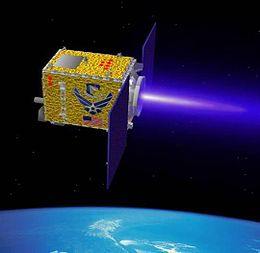
\includegraphics[height=2.7cm]{XSS11.jpg}\hspace*{0.2cm}
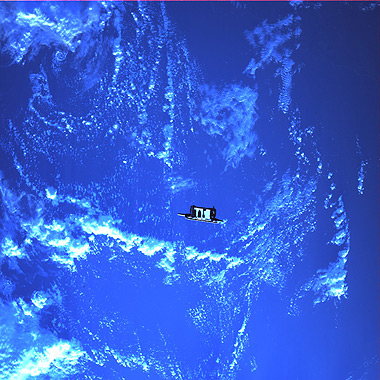
\includegraphics[height=2.7cm]{DLRPrisma.jpg}\hspace*{0.2cm}
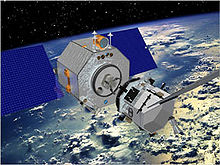
\includegraphics[height=2.7cm]{OrbitalExpress.jpg}}
\centerline{\scriptsize\selectfont
AFRL XSS-11\hspace*{1.5cm} DLR PRISMA\hspace*{1.5cm} DARPA Orbital Express}
\end{frame}


\begin{frame}
\frametitle{Introduction}

\begin{itemize}
\item Space-Based Space Surveillance (SBSS)
	\begin{itemize}
	\item Detection, collection, identification and tracking of man-made space objects from deep space to low-earth orbits
%	\item Ground-based optical systems are limited to clear weather, night-time observations
	\item SBSS provides all-weather, day and night, near real-time space situation awareness data
	\item Ability to search for lost/unknown space objects in deep space
	\end{itemize}
	\vspace*{0.3cm}\pause
\item Relative Orbit Determination with \Emph{Angles-Only Measurements}
	\begin{itemize}
	\item Lines-of-sight between satellites are measured by optical sensors
	\item Optical sensors have desirable properties of low-cost and minimal mainternance
	\item Range is not available:\\ \Emph{Unobservable for linearized relative orbital dynamics} [Woffinden 09]
	\item Observability for nonlinear relative orbital dynamics has been unknown
	\end{itemize}
\end{itemize}

\vspace*{0.3cm}\pause
    \centerline{
    \begin{beamercolorbox}[wd=10.68cm,sep=0.2cm,center,shade=on]{numerical}
        \small\bfseries\selectfont Goal: Investigative Observability for \textit{Nonlinear} Relative Orbital Dynamics
    \end{beamercolorbox}}

\end{frame}

\section*{}
\subsection*{II. Problem Formulation}


\begin{frame}
\frametitle{Relative Orbit Dynamics}

\begin{columns}
\begin{column}{6.5cm}
\footnotesize\selectfont
\only<1>{
\setlength{\unitlength}{1cm}
\begin{picture}(7,7)(0,0)
\put(0,0){\includegraphics[width=7cm]{PF0.pdf}}
\put(3.2,1.3){$a$}
\put(4.8,2.8){Chief}
\end{picture}
}
\only<2>{
\setlength{\unitlength}{1cm}
\begin{picture}(7,7)(0,0)
\put(0,0){\includegraphics[width=7cm]{PF1.pdf}}
\put(3.2,1.3){$a$}
\put(6.15,3.55){$x$}
\put(4.5,4.5){$y$}
\put(4.8,2.8){Chief}
\end{picture}
}
\only<3>{
\setlength{\unitlength}{1cm}
\begin{picture}(7,7)(0,0)
\put(0,0){\includegraphics[width=7cm]{PF2.pdf}}
\put(3.2,1.3){$a$}
\put(6.15,3.55){$x$}
\put(4.5,4.5){$y$}
\put(5.7,4.3){$\mathbf{r}$}
\put(4.8,2.8){Chief}
\put(5.3,6.1){Deputy}
\end{picture}
}
\end{column}
%
\begin{column}{6cm}
\begin{itemize}
\item Chief Satellite
	\begin{itemize}
	\item On a circular orbit
	\item Orbital radius $a$ is known
	\end{itemize}
\vspace*{0.3cm}\pause
\item Local-vertical, local-horizontal (LVLH) frame
	\begin{itemize}
	\item $x$--axis: radial
	\item $y$--axis: tangent to the path
	\item $z$--axis: normal to the orbital plane
	\item Rotating about the $z$--axis with $\mathbf{\omega}=\sqrt{\frac{\mu}{a^3}}$.
	\end{itemize}
\vspace*{0.3cm}\pause
\item Deputy Satellite
	\begin{itemize}
	\item On an unknown, arbitrary orbit\\
	\item Relative position $\mathbf{r}\in\Re^3$

	\end{itemize}
\end{itemize}
\end{column}
\end{columns}
\end{frame}


\begin{frame}
\frametitle{Relative Orbit Dynamics}

\begin{itemize}
\item Nonlinear Equations of Motion (Two-Body Gravity Only)
	\begin{itemize}
	\item State vector: $\mathbf{x}=[\r,\;\dot\r]\in\Re^6$
	\item State equation: $\dot \x = f(\x)$, where
\begin{align*}
f(\mathbf{x}) 
=\begin{bmatrix}
\dot \r \\
-2\omega\times \dot\r - \omega\times(\omega\times \r_a) -\dfrac{\mu \r_a}{\|\r_a\|^3}
\end{bmatrix}.
\end{align*}
($\r_a=\r+[a,0,0]^T$: position vector of deputy from the center of Earth)
	\end{itemize}
\vspace*{0.3cm}\pause
\item Hill-Clohessey-Wiltshire (HCW) Equations
	\begin{itemize}
	\item Linearization of above ODEs about $\x=0$: $\delta\dot\x = A\delta \x$, where
\begin{align*}
A=\deriv{f(\x)}{\x}\bigg|_{\x=0}
=\begin{bmatrix}
0 & 0 & 0 & 1 & 0 & 0\\
0 & 0 & 0 & 0 & 1 & 0\\
0 & 0 & 0 & 0 & 0 & 1\\
3n^2 & 0 & 0 & 0 & 2n & 0\\
0 & 0 & 0 & -2n & 0 & 0\\
0 & 0 & -n^2 & 0 & 0 & 0
\end{bmatrix}.
\end{align*}
	\end{itemize}
\end{itemize}
\end{frame}



\begin{frame}
\frametitle{Line-of-sight Measurements}

\begin{columns}
\begin{column}{6.5cm}
\footnotesize\selectfont
\setlength{\unitlength}{1cm}
\begin{picture}(7,7)(0,0)
\put(0,0){\includegraphics[width=7cm]{PF3.pdf}}
\put(3.2,1.3){$a$}
\put(6.15,3.55){$x$}
\put(4.5,4.5){$y$}
\put(5.6,4.0){$\y$}
\put(4.8,2.8){Chief}
\put(5.3,6.1){Deputy}
\end{picture}
\end{column}
%
\begin{column}{6cm}
\begin{itemize}
\item Measurements
	\begin{itemize}
	\item Line-of-sight from chief to deputy is measured
	\item Measurement:
	\begin{align*}
	\y = \frac{\r}{\|\r\|}\in\Re^3
	\end{align*}
	(unit-length: $\|\y\|$=1)
	\end{itemize}
\vspace*{0.3cm}\pause
\item Relative Orbit Determination
	\begin{itemize}
	\item Wish to determine the relative orbit $\x=[\r,\dot\r]$ completely from $\y(t)$ only
	\end{itemize}	
\end{itemize}	
\end{column}
\end{columns}
\end{frame}

\section*{}
\subsection*{III. Observability}


\begin{frame}
\frametitle{Observability of HCW Equations}

\begin{itemize}
\item Solution of the Linear HCW Equation
	\begin{itemize}
	\item Let $\x(t)$ be the solution with an initial condition $\x(t_0)=\x_0$.
	\begin{align*}
	\x(t) = \exp(A(t-t_0)) \x_0
	\end{align*}
	\item \Emph{Homogeneity property}: let $\x'(t)$ be the solution with a \textit{scaled} initial condition $\x'(t_0)=\alpha\x_0$ for any $\alpha\in\Re$, then 
	\begin{align*}
	\x'(t) = \exp(A(t-t_0)) (\alpha\x_0) = \alpha \x(t).
	\end{align*}
	\end{itemize}
\vspace*{0.3cm}\pause
\item Observability of the HCW Equation with Angles-Only Measurements
	\begin{itemize}
	\item The two distinct relative orbits $\x(t)=[\r(t),\dot\r(t)]$ and $\x'(t)=[\r'(t),\dot\r'(t)]$ yield the \Emph{identical} line-of-sight measurements:
	\begin{align*}
	\y(t)=\frac{\r(t)}{\|\r(t)\|},\quad \y'(t)=\frac{\r'(t)}{\|\r'(t)\|}=\frac{\alpha\r(t)}{\|\alpha\r(t)\|}\equiv\y(t).
	\end{align*}
	\end{itemize}
\end{itemize}

\vspace*{0.2cm}\pause
    \centerline{
    \begin{beamercolorbox}[wd=10.68cm,sep=0.2cm,center,shade=on]{numerical}
        \small\bfseries\selectfont Linearized relative orbit is NOT observable with angles-only measurements!
    \end{beamercolorbox}}

\end{frame}


\begin{frame}
\frametitle{Observability of Nonlinear Systems}

\begin{itemize}
\item Observability Concepts 
	\begin{itemize}
	\item Nonlinear system: 
	\begin{align*}\dot \x =f(\x)\in\Re^N,\qquad \y=h(\x)\in\Re^M\end{align*}
	\item A pair of states $\x_0$ and $\x_1$ is \Emph{\textit{indistinguishable}} if the outputs of the corresponding solutions starting from $\x_0$ and $\x_1$ are identical. 
	\item The system is \Emph{\textit{locally weakly observable at $\x_0$}}, if there exists an open neighborhood $U$ of $\x_0$ such that the only indistinguishable point to $\x_0$ in $U$ is the point $\x_0$ itself. 
	\end{itemize}
\vspace*{0.3cm}\pause
\item Observability Criteria  {\small\selectfont [Hermann, Krener 1977]}
	\begin{itemize}
	\item Lie-derivative: $L_f h(\x) = \deriv{h(\x)}{\x}f(\x)=\dot h(\x)\in\Re^{M}$.
	\item Observability Matrix
	\begin{align*}
\mathcal{O}(\x_0) = \deriv{}{\x} \begin{bmatrix} h(\x) \\ L_f^1 h(\x)\\ \vdots \\L_f^{N-1} h(\x)\end{bmatrix}\bigg|_{\x=\x_0}\in\Re^{NM\times N}.
\end{align*}
	\item The system is \Emph{\textit{locally weakly observable at $\x_0$}} if \Emph{$\mathrm{rank}[\mathcal{O}(\x_0)]= N$}.
	\end{itemize}
\end{itemize}
\end{frame}



\begin{frame}
\frametitle{Observability of Nonlinear Relative Orbits}

\begin{itemize}
\item Observability Matrix {\footnotesize\selectfont (up to the second order Lie derivative)}
\begin{align}
\mathcal{O} =
\begin{bmatrix}
\deriv{\y}{\r} & \deriv{\y}{\dot\r}\\
\deriv{\dot\y}{\r} & \deriv{\dot\y}{\dot\r}\\
\deriv{\ddot\y}{\r} & \deriv{\ddot\y}{\dot\r}
\end{bmatrix}
\triangleq
\begin{bmatrix}
\mathcal{O}_{00} & 0_{3\times 3}\\
\mathcal{O}_{10} & \mathcal{O}_{11}\\
\mathcal{O}_{20} & \mathcal{O}_{21}
\end{bmatrix}\in\Re^{9\times 6},
\end{align}
\only<1>{\scriptsize\selectfont where
\begin{align*}
\mathcal{O}_{00} & = \deriv{\y}{\r} = \frac{1}{\|\r\|}(I - \y\y^T),\\
\mathcal{O}_{10} & = \deriv{\dot\y}{\r} = \deriv{}{\r} \parenth{\deriv{\y}{\r}\dot \r}= -\frac{1}{\|\r\|^2}\braces{
{\dot\r\y^T +\y^T\dot\r I +\y\dot\r^T}
- 3\y\y^T\dot\r \y^T},\\
\mathcal{O}_{11} & = \deriv{\dot\y}{\dot\r} = \deriv{}{\dot\r} \parenth{\deriv{\y}{\r}\dot \r}= \deriv{\y}{\r} = \mathcal{O}_{00},\\
\mathcal{O}_{20} & = \deriv{\ddot\y}{\r} = -\dfrac{2\dot\r \dot\r^T  +\dot\r^T\dot\r I}{\|\r\|^3}
+3\dfrac{2(\r^T\dot\r) \dot\r\r^T +(\dot\r^T\dot\r)\r\r^T
+(\r^T\dot\r)^2 I
+2(\r^T\dot\r)\r  \dot\r^T
}{\|\r\|^5}
- 15 \dfrac{(\r^T\dot\r)^2\r  \r^T}{\|\r\|^7}\nonumber \\
&\quad -\dfrac{\ddot{\r}\r^T +\r^T\ddot{\r} I +\r \ddot{\r}^T}{\|\r\|^3}
+ 3 \dfrac{(\r^T\ddot{\r})\r \r^T}{\|\r\|^5}
+\parenth{\dfrac{I}{\|\mathbf{r}\|} - \dfrac{\mathbf{r}\mathbf{r}^T}{\|\mathbf{r}\|^3}}
\parenth{-[\omega]_\times^2 -\dfrac{\mu I_{3\times 3}}{\|\r_a\|^3} + \dfrac{3\mu\r_a\r_a^T}{\|\r_a\|^5}},\\
\mathcal{O}_{21} & = \deriv{\ddot\y}{\dot\r} = \deriv{}{\dot\r}\parenth{\deriv{}{\r}\parenth{\deriv{\y}{\r}\dot\r}\dot\r + \deriv{\y}{\r}\ddot\r} = 2 \deriv{}{\r} \parenth{\deriv{\y}{\r}\dot\r} + \deriv{\y}{\r} \deriv{\ddot\r}{\dot\r}
= 2\mathcal{O}_{10} 
- 2 \mathcal{O}_{00}[\omega]_\times,
\vspace*{-0.7cm}\end{align*}
(These expressions have been verified by \Emph{Matlab Symbolic Computation Toolbox})}
%
\only<2>{\scriptsize\selectfont They satisfy the following identities:
\begin{align*}
\mathcal{O}_{10}\r & = 
-\mathcal{O}_{00}\dot\r,\label{eqn:O10r}\\
\mathcal{O}_{10}\dot\r & = -\frac{1}{\|\r\|^2}\braces{
{2\dot\r(\y^T\dot \r)  +\y(\dot\r^T\dot \r)}
- 3\y(\y^T\dot\r)^2},\label{eqn:O10dotr}\\
\mathcal{O}_{20}\r %& = 
& = -2\mathcal{O}_{10}\dot\r +\mathcal{O}_{00}\braces{-\ddot \r +\deriv{\ddot\r}{\r}\r},\label{eqn:O20r}\\
\mathcal{O}_{21}\r & = -2\mathcal{O}_{00} (\dot\r+\omega\times\r),\label{eqn:O21r}\\
\mathcal{O}_{21}\dot\r & = 2\mathcal{O}_{10} \dot\r
- 2 \mathcal{O}_{00}[\omega]_\times\dot\r,\label{eqn:O21rdot}
\end{align*}
which are useful to derive the observability criteria.}
\end{itemize}
\end{frame}


\begin{frame}
\frametitle{Observability of Nonlinear Relative Orbits}

\begin{theorem}[Sufficient Conditions for Observability]
Define three vectors $\mathbf{v}_{rel}$, $\mathbf{a}_1,\mathbf{a}_2\in\Re^3$ as 
\begin{align}
\mathbf{v}_{rel} & = \dot\r +\omega\times\r,\label{eqn:vrel}\\
\mathbf{a}_1 & = \ddot\r-\deriv{\ddot\r}{\r}\r = -2\omega\times \dot\r - [\omega]_\times^2 a \mathbf{e}_1 -\dfrac{\mu a }{\|\r_a\|^3}\mathbf{e}_1- \dfrac{3\mu\r_a^T\r}{\|\r_a\|^5}\r_a,\label{eqn:a1}\\
\mathbf{a}_2 & = \ddot\r-\deriv{\ddot\r}{\r}\r -\deriv{\ddot\r}{\dot\r}\dot\r = \mathbf{a}_1+2\omega\times\dot\r.\label{eqn:a2}
\end{align}
The nonlinear relative orbital dynamics is locally weakly observable at $\x=[\r^T,\dot\r^T]$ if
%\begin{list}{}{\setlength{\leftmargin}{1cm}\setlength{\itemsep}{0mm}\setlength{\parsep}{0mm}\setlength{\topsep}{0mm}\setlength{\parskip}{0mm}\setlength{\labelwidth}{2cm}}
%\item[(i)] when $\r\times\dot\r =0$, $\r\times\mathbf{a}_1\neq 0$ and $\r^T(\mathbf{v}_{ref}\times \mathbf{a}_1)\neq 0$,
%\item[(ii)] when $\r\times\dot\r \neq 0$, $\r\times\mathbf{a}_2\neq 0$ and $\r^T(\mathbf{v}_{ref}\times \mathbf{a}_2)\neq 0$.
%\end{list}
\begin{align}
(i)\; &\text{when $\r\times\dot\r =0$, $\r\times\mathbf{v}_{rel}\neq0$, $\r\times\mathbf{a}_1\neq 0$,  and $\r^T(\mathbf{v}_{ref}\times \mathbf{a}_1)\neq 0$},\label{eqn:cond1}\\
(ii)\; &\text{when $\r\times\dot\r \neq 0$, $\r\times\mathbf{v}_{rel}\neq0$, $\r\times\mathbf{a}_2\neq 0$ and $\r^T(\mathbf{v}_{ref}\times \mathbf{a}_2)\neq 0$.}\label{eqn:cond2}
\end{align}
\end{theorem}

\vspace*{0.2cm}\pause
    \centerline{
    \begin{beamercolorbox}[wd=11.5cm,sep=0.2cm,center,shade=on]{numerical}
        \small\bfseries\selectfont Nonlinear relative orbits are OBSERVABLE under certain geometric conditions!
    \end{beamercolorbox}}

\end{frame}


\begin{frame}
\frametitle{Observability of Nonlinear Relative Orbits}

\begin{itemize}
\item Sufficient condition: $\r\times\mathbf{v}_{rel}\neq0$
	\begin{itemize}
	\item $\mathbf{v}_{rel} = \dot\r +\omega\times\r$: relative velocity in the inertial frame
	\item violated if deputy is flying directly toward or away from chief
	\end{itemize}
	\vspace*{0.3cm}\pause
\item Sufficient condition: $\r\times\mathbf{a}_1\neq 0$ (or $\r\times\mathbf{a}_2\neq 0$)
	\begin{itemize}
	\item $\mathbf{a}_1 = \ddot\r-\deriv{\ddot\r}{\r}\r$: difference between acceleration and its variation along $\r$
	\item satisfied in general as $\mathbf{a}_1$ (or $\mathbf{a}_2$) is pretty arbitrary
	\end{itemize}
	\vspace*{0.3cm}\pause
\item Sufficient condition: $\r^T(\mathbf{v}_{ref}\times \mathbf{a}_1)\neq 0$ (or $\r^T(\mathbf{v}_{ref}\times \mathbf{a}_2)\neq 0$)
	\begin{itemize}
	\item The (signed) volume of the \textit{parallelepiped} defined by $\r$, $\mathbf{v}_{rel}$, and $\mathbf{a}_1$ (or $\mathbf{a}_2$)
	
	\centerline{\setlength{\unitlength}{1cm}\footnotesize\selectfont
	\begin{picture}(3,2.2)(0,0)
	\only<3>{
	\put(0,0){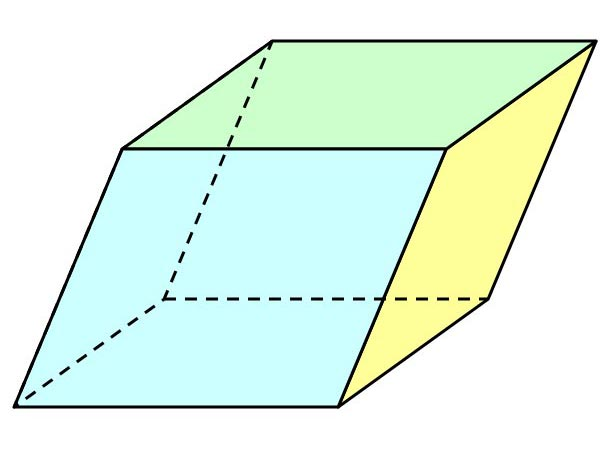
\includegraphics[width=3cm]{pp.jpg}}}
	\put(1.,0.25){$\r$}
	\put(0.5,0.6){$\mathbf{v}_{rel}$}
	\put(0.2,0.9){$\mathbf{a}$}
	\end{picture}}
	\item violated for planar relative orbits
	\end{itemize}
	
\end{itemize}

\end{frame}


\section*{}
\subsection*{IV. Numerical Example}

\begin{frame}
\frametitle{Numerical Examples}

\begin{itemize}
\item Orbital Properties
	\begin{itemize}
	\item Chief: an equatorial circular orbit with an orbital altitude of $500\,\mathrm{km}$
	\item Deputy
		\begin{itemize}
		\item Semi-major axis is chosen such that its orbital period is same as chief,\\
		resulting in \textit{periodic relative orbits}.
		\item Eccentricity is fixed at $e_{deputy}=0.2$
		\item Inclination is varied as $i_{deputy}=0^\circ,\, 10^\circ,\, \ldots 50^\circ$
		\end{itemize}
	\end{itemize}
\vspace*{0.3cm}\pause
\item Performance Metrics
	\begin{itemize}
	\item Min-singular value and condition number of $\mathcal{O}$ are computed
	\item Extended Kalman filter is developed
		\begin{itemize}
		\item Initial estimate: $\hat\x(0)=2\x(0)$
		\item Two candidate error measures
\begin{align*}
e_{dir}  & = \sqrt{\frac{1}{N}\sum_{k=0}^N\parenth{\cos^{-1}\parenth{\frac{\mathbf{x}(t_k)^T \hat{\mathbf{x}} (t_k)}
{\|\mathbf{x}(t_k)\| \|\hat{\mathbf{x}} (t_k)\|}}}^2}\\
e_{mag}  & = \sqrt{\frac{1}{N}\sum_{k=0}^N\parenth{
\frac{\|\mathbf{x}(t_k)\|-\|\hat{\mathbf{x}} (t_k)\|}{\|\mathbf{x}(t_k)\|}}^2}
\end{align*}
		\end{itemize}
	\end{itemize}	
\end{itemize}

\end{frame}

\begin{frame}
\frametitle{Numerical Examples}
\framesubtitle{Deputy inclination $i=0^\circ$}

\begin{figure}
\only<1>{
\centerline{
	\subfigure[Trajectory in the inertial frame]{
		\includegraphics[width=0.5\columnwidth]{ISSFD14_i_0_OT_iner.pdf}}
	\hspace*{0.05\textwidth}
	\subfigure[Relative trajectory in the LVLH frame]{
		\includegraphics[width=0.5\columnwidth]{ISSFD14_i_0_OT_lvlh.pdf}}
}}
\only<2>{
\centerline{
	\subfigure[Min. singular value of $\mathcal{O}$]{
		\includegraphics[width=0.5\columnwidth]{ISSFD14_i_0_OT_sig.pdf}}
	\hspace*{0.05\textwidth}
	\subfigure[Condition number of $\mathcal{O}$]{
		\includegraphics[width=0.5\columnwidth]{ISSFD14_i_0_OT_cond.pdf}}
}}
\only<3>{
\centerline{
	\subfigure[Estimation errors]{
		\includegraphics[width=0.5\columnwidth]{PE_i_0_e.pdf}}
	\hspace*{0.05\textwidth}
	\subfigure[True $\|\x\|$ (red) and Estimated $\|\hat\x\|$ (blue)]{
		\includegraphics[width=0.5\columnwidth]{PE_i_0_xx_norm.pdf}}
}}
\end{figure}
\end{frame}


\begin{frame}
\setcounter{subfigure}{0}
\frametitle{Numerical Examples}
\framesubtitle{Deputy inclination $i=10^\circ$}

\begin{figure}
\only<1>{
\centerline{
	\subfigure[Trajectory in the inertial frame]{
		\includegraphics[width=0.5\columnwidth]{ISSFD14_i_10_OT_iner.pdf}}
	\hspace*{0.05\textwidth}
	\subfigure[Relative trajectory in the LVLH frame]{
		\includegraphics[width=0.5\columnwidth]{ISSFD14_i_10_OT_lvlh.pdf}}
}}
\only<2>{
\centerline{
	\subfigure[Min. singular value of $\mathcal{O}$]{
		\includegraphics[width=0.5\columnwidth]{ISSFD14_i_10_OT_sig.pdf}}
	\hspace*{0.05\textwidth}
	\subfigure[Condition number of $\mathcal{O}$]{
		\includegraphics[width=0.5\columnwidth]{ISSFD14_i_10_OT_cond.pdf}}
}}
\only<3>{
\centerline{
	\subfigure[Estimation errors]{
		\includegraphics[width=0.5\columnwidth]{PE_i_10_e.pdf}}
	\hspace*{0.05\textwidth}
	\subfigure[True $\|\x\|$ (red) and Estimated $\|\hat\x\|$ (blue)]{
		\includegraphics[width=0.5\columnwidth]{PE_i_10_xx_norm.pdf}}
}}
\end{figure}
\end{frame}


%\begin{frame}
%\setcounter{subfigure}{0}
%\frametitle{Numerical Examples}
%\framesubtitle{Deputy inclination $i=20^\circ$}
%
%\begin{figure}
%\only<1>{
%\centerline{
%	\subfigure[Trajectory in the inertial frame]{
%		\includegraphics[width=0.5\columnwidth]{ISSFD14_i_20_OT_iner.pdf}}
%	\hspace*{0.05\textwidth}
%	\subfigure[Relative trajectory in the LVLH frame]{
%		\includegraphics[width=0.5\columnwidth]{ISSFD14_i_20_OT_lvlh.pdf}}
%}}
%\only<2>{
%\centerline{
%	\subfigure[Min. singular value of $\mathcal{O}$]{
%		\includegraphics[width=0.5\columnwidth]{ISSFD14_i_20_OT_sig.pdf}}
%	\hspace*{0.05\textwidth}
%	\subfigure[Condition number of $\mathcal{O}$]{
%		\includegraphics[width=0.5\columnwidth]{ISSFD14_i_20_OT_cond.pdf}}
%}}
%\only<3>{
%\centerline{
%	\subfigure[Estimation errors]{
%		\includegraphics[width=0.5\columnwidth]{PE_i_20_e.pdf}}
%	\hspace*{0.05\textwidth}
%	\subfigure[True $\|\x\|$ (red) and Estimated $\|\hat\x\|$ (blue)]{
%		\includegraphics[width=0.5\columnwidth]{PE_i_20_xx_norm.pdf}}
%}}
%\end{figure}
%\end{frame}


\begin{frame}
\setcounter{subfigure}{0}
\frametitle{Numerical Examples}
\framesubtitle{Deputy inclination $i=30^\circ$}

\begin{figure}
\only<1>{
\centerline{
	\subfigure[Trajectory in the inertial frame]{
		\includegraphics[width=0.5\columnwidth]{ISSFD14_i_30_OT_iner.pdf}}
	\hspace*{0.05\textwidth}
	\subfigure[Relative trajectory in the LVLH frame]{
		\includegraphics[width=0.5\columnwidth]{ISSFD14_i_30_OT_lvlh.pdf}}
}}
\only<2>{
\centerline{
	\subfigure[Min. singular value of $\mathcal{O}$]{
		\includegraphics[width=0.5\columnwidth]{ISSFD14_i_30_OT_sig.pdf}}
	\hspace*{0.05\textwidth}
	\subfigure[Condition number of $\mathcal{O}$]{
		\includegraphics[width=0.5\columnwidth]{ISSFD14_i_30_OT_cond.pdf}}
}}
\only<3>{
\centerline{
	\subfigure[Estimation errors]{
		\includegraphics[width=0.5\columnwidth]{PE_i_30_e.pdf}}
	\hspace*{0.05\textwidth}
	\subfigure[True $\|\x\|$ (red) and Estimated $\|\hat\x\|$ (blue)]{
		\includegraphics[width=0.5\columnwidth]{PE_i_30_xx_norm.pdf}}
}}
\end{figure}
\end{frame}


%\begin{frame}
%\setcounter{subfigure}{0}
%\frametitle{Numerical Examples}
%\framesubtitle{Deputy inclination $i=40^\circ$}
%
%\begin{figure}
%\only<1>{
%\centerline{
%	\subfigure[Trajectory in the inertial frame]{
%		\includegraphics[width=0.5\columnwidth]{ISSFD14_i_40_OT_iner.pdf}}
%	\hspace*{0.05\textwidth}
%	\subfigure[Relative trajectory in the LVLH frame]{
%		\includegraphics[width=0.5\columnwidth]{ISSFD14_i_40_OT_lvlh.pdf}}
%}}
%\only<2>{
%\centerline{
%	\subfigure[Min. singular value of $\mathcal{O}$]{
%		\includegraphics[width=0.5\columnwidth]{ISSFD14_i_40_OT_sig.pdf}}
%	\hspace*{0.05\textwidth}
%	\subfigure[Condition number of $\mathcal{O}$]{
%		\includegraphics[width=0.5\columnwidth]{ISSFD14_i_40_OT_cond.pdf}}
%}}
%\only<3>{
%\centerline{
%	\subfigure[Estimation errors]{
%		\includegraphics[width=0.5\columnwidth]{PE_i_40_e.pdf}}
%	\hspace*{0.05\textwidth}
%	\subfigure[True $\|\x\|$ (red) and Estimated $\|\hat\x\|$ (blue)]{
%		\includegraphics[width=0.5\columnwidth]{PE_i_40_xx_norm.pdf}}
%}}
%\end{figure}
%\end{frame}


\begin{frame}
\setcounter{subfigure}{0}
\frametitle{Numerical Examples}
\framesubtitle{Deputy inclination $i=50^\circ$}

\begin{figure}
\only<1>{
\centerline{
	\subfigure[Trajectory in the inertial frame]{
		\includegraphics[width=0.5\columnwidth]{ISSFD14_i_50_OT_iner.pdf}}
	\hspace*{0.05\textwidth}
	\subfigure[Relative trajectory in the LVLH frame]{
		\includegraphics[width=0.5\columnwidth]{ISSFD14_i_50_OT_lvlh.pdf}}
}}
\only<2>{
\centerline{
	\subfigure[Min. singular value of $\mathcal{O}$]{
		\includegraphics[width=0.5\columnwidth]{ISSFD14_i_50_OT_sig.pdf}}
	\hspace*{0.05\textwidth}
	\subfigure[Condition number of $\mathcal{O}$]{
		\includegraphics[width=0.5\columnwidth]{ISSFD14_i_50_OT_cond.pdf}}
}}
\only<3>{
\centerline{
	\subfigure[Estimation errors]{
		\includegraphics[width=0.5\columnwidth]{PE_i_50_e.pdf}}
	\hspace*{0.05\textwidth}
	\subfigure[True $\|\x\|$ (red) and Estimated $\|\hat\x\|$ (blue)]{
		\includegraphics[width=0.5\columnwidth]{PE_i_50_xx_norm.pdf}}
}}
\end{figure}
\end{frame}


\begin{frame}
\frametitle{Numerical Examples}

\begin{table}[h]
\caption{Estimation error compared with singularity of observability matrix}\label{tab:SVD}
\begin{center}
\begin{tabularx}{0.87\textwidth}{*{5}{>{$}c<{$}}}\toprule
i_{deputy} & \text{min} \braces{\sigma(\mathcal{O})} & \mathrm{cond}\braces{\mathcal{O}} 
& e_{dir} \;(\mathrm{rad}) & {e_{mag}} \;(\mathrm{unitless}) \\\midrule
0^\circ & 10^{-19.3041} & 10^{15.9893} & 0.0211  & {0.3361} \\
10^\circ & 10^{-10.3766} & 10^{7.0369} & 0.0172  & {0.2204} \\
20^\circ & 10^{-10.2584} & 10^{6.8603} & 0.0187  & {0.1681} \\
30^\circ & 10^{-10.2290} & 10^{6.7634} & 0.0248  & {0.1596} \\
40^\circ & 10^{-10.2176} & 10^{6.6873} & 0.0421  & {0.1703} \\
50^\circ & 10^{-10.2155} & 10^{6.6273} & 0.0599  & {0.1841} \\\bottomrule
\end{tabularx}
\end{center}
\end{table}
\end{frame}

\section*{}
\subsection*{V. Conclusions}

\begin{frame}
\frametitle{Conclusions}

\begin{itemize}
\item Determination of Relative Orbits with Angles-Only Measurements
	\begin{itemize}
	\item Chief is on a circular orbit with known orbital properties
	\item Deputy is on an arbitrary, unknown orbit
	\item Line-of-sight from chief to deputy is measured
	\end{itemize}
	\vspace*{0.3cm}\pause
\item Nonlinear Observability of Deputy
	\begin{itemize}
	\item It is well-known that the orbital properties of deputy are unobservable for the linearized relative orbital dynamics, represented by the HCW equations
	\item In this paper, we have shown that deputy is \Emph{observable with angles-only measurements} under certain geometric conditions along the \Emph{nonlinear relative orbital dynamics}
	\item Observability is illustrated by extended Kalman filter
	\end{itemize}
	\vspace*{0.3cm}\pause
\item Future Works
	\begin{itemize}
	\item Observability criteria based on higher-order Lie-derivatives
	\item Introduce nonlinear observability measure\\
	(nonlinear Gramian-like measure studied in 2013)
	\item Numerical studies including orbital perturbations
	\end{itemize}
\end{itemize}
\end{frame}
\end{document}






















